\chapter{Manufacturing of Planar Detectors}
The manufacturing process of a planar HPGe detector begins with a slice from a crystal boule that has been tested for quality and is know to be detector grade.
Typical boules slices are solid discs that can range from a few millimeters up to several centimeters in thickness and 5+ centimeters in diameter.
This large size allows for several detector samples to be cut from each slice so careful geometry considerations are important in order to minimize wasted material.
The goal is for the detector sample to look approximately like figure \ref{fig:dummydet} which is an example of a planar detector with so called top hat geometry.
\begin{figure}[htpb]
\centering
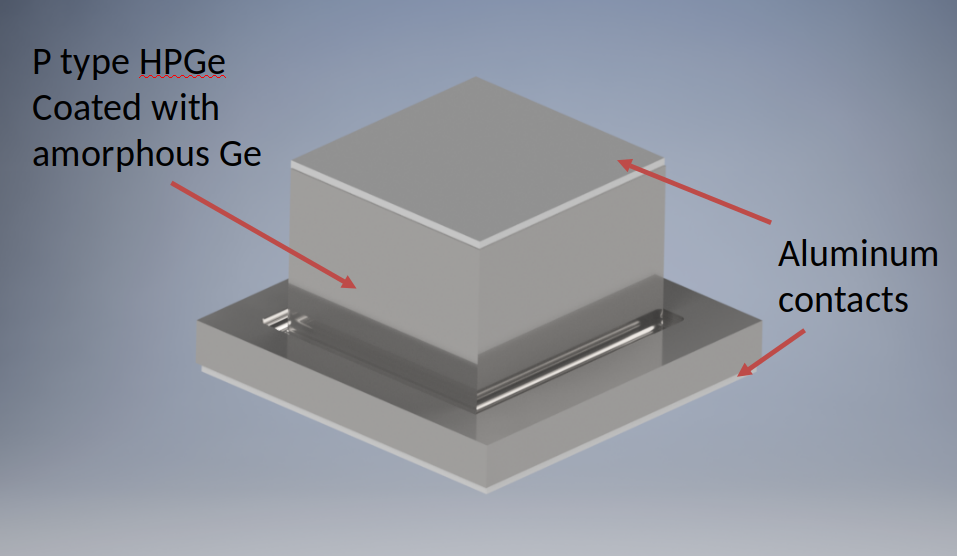
\includegraphics[width=0.5\textwidth]{dummy-det}
\caption{Example detector geometry with four wings}
\label{fig:dummydet}
\end{figure}
The brims of the hat are called wings and serve as a dead area of the detector for handling during the manufacturing process.
The detector is not required to be perfectly square to work so length and width can vary within a few centimeters.
What is of importance are the overall thickness and that the top and bottom faces are parallel.
Due to the relatively long mean free path of gamma rays in germanium, a detector should aim to be at least one centimeter thick.

Once considerations for geometry have been made, the detector manufacturing process begins.
To start, the germanium boule slice is cut into several rectangular cubes.
Then, work proceeds using one of the cubes, saving the rest for the next time.
\section{Mechanical Processing}

\begin{figure}[htpb]
\centering
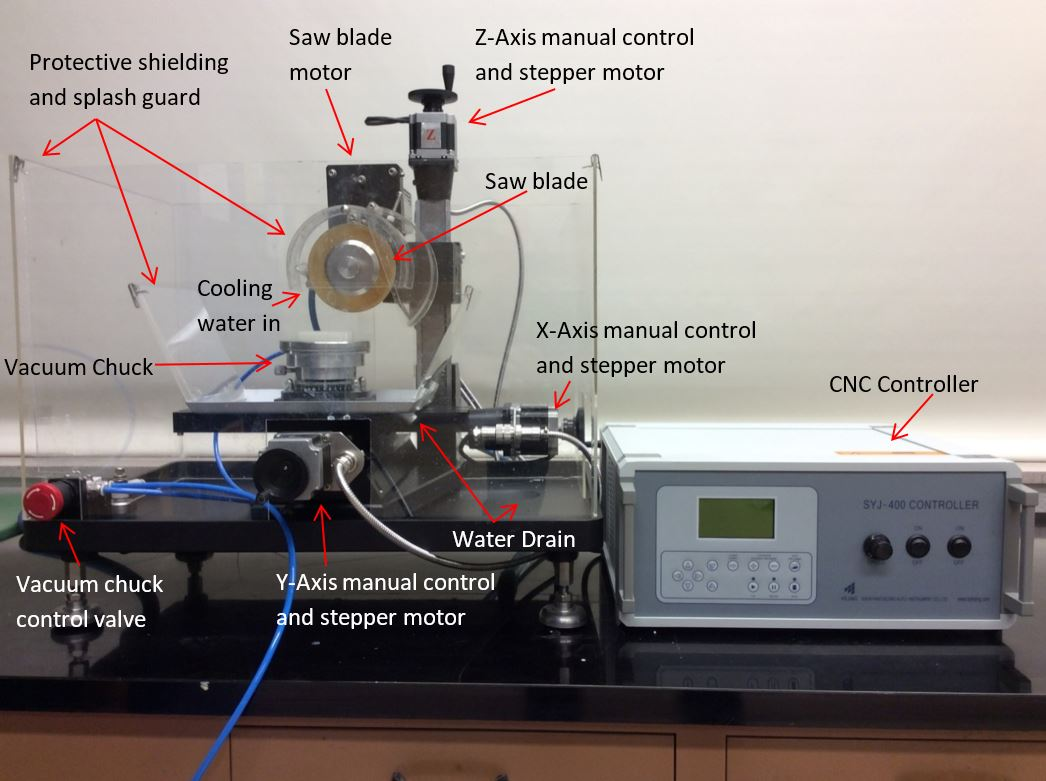
\includegraphics[width=0.5\textwidth]{diamond-saw.jpg}
\caption{The diamond saw used to cut boules into detector samples.}
\label{fig:diamondsaw}
\end{figure}

\begin{figure}[htpb]
\centering
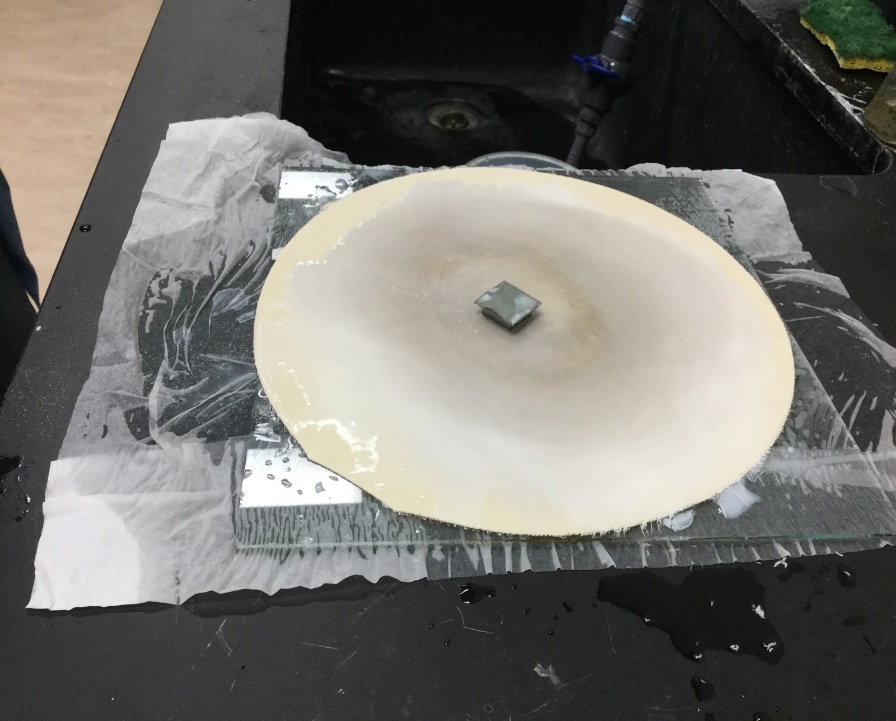
\includegraphics[width=0.5\textwidth]{lapping.jpg}
\caption{An example of lapping the detector sample}
\label{fig:lapping}
\end{figure}

\section{Chemical Processing}

\begin{figure}[htpb]
\centering
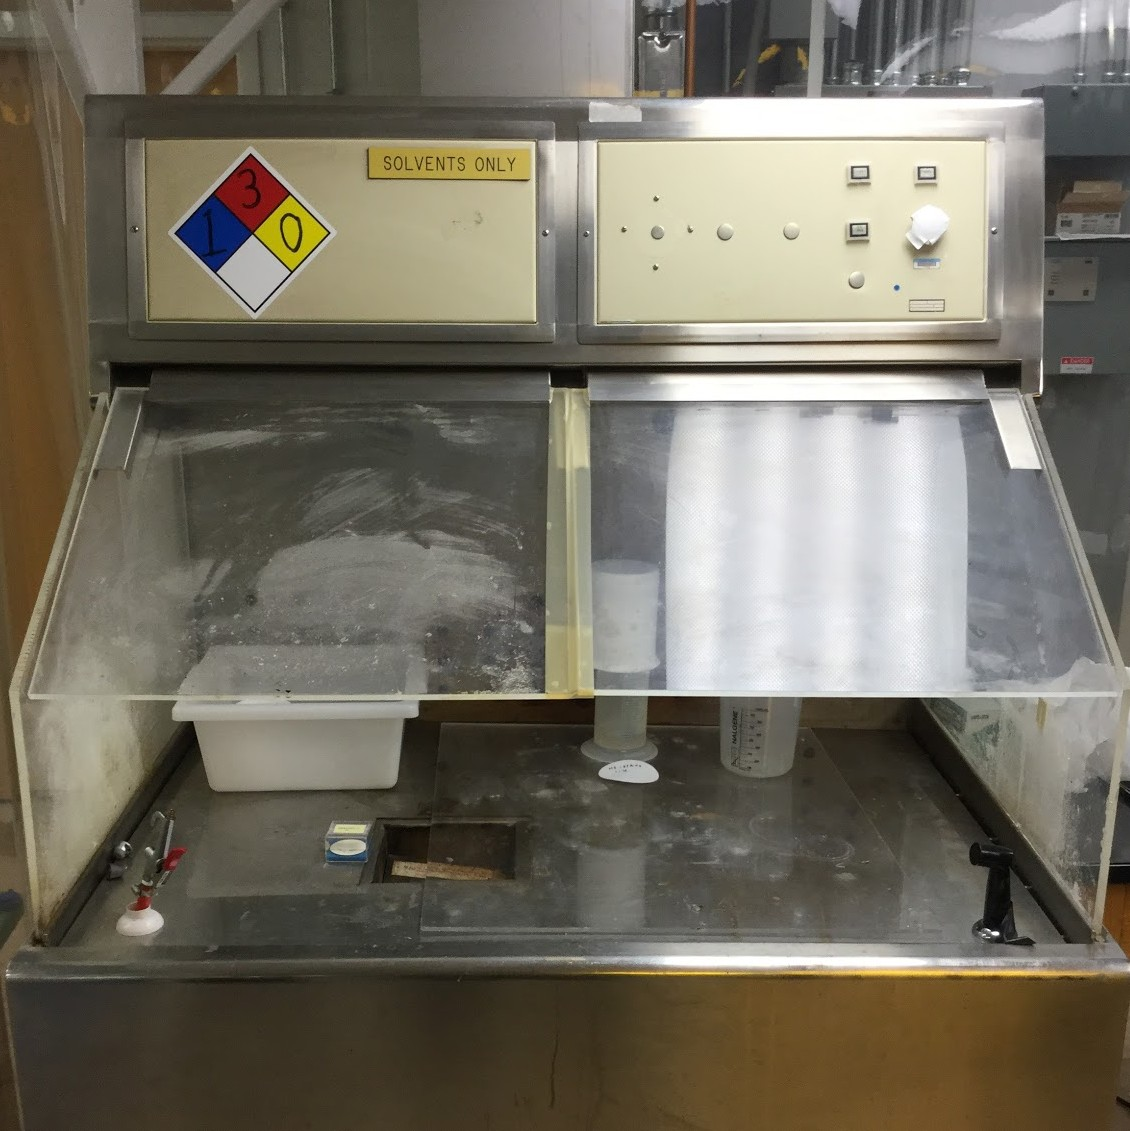
\includegraphics[width=0.5\textwidth]{metal-hood.jpg}
\caption{Metal hood for use with solvents}
\label{fig:metalhood}
\end{figure}


\begin{figure}[htpb]
\centering
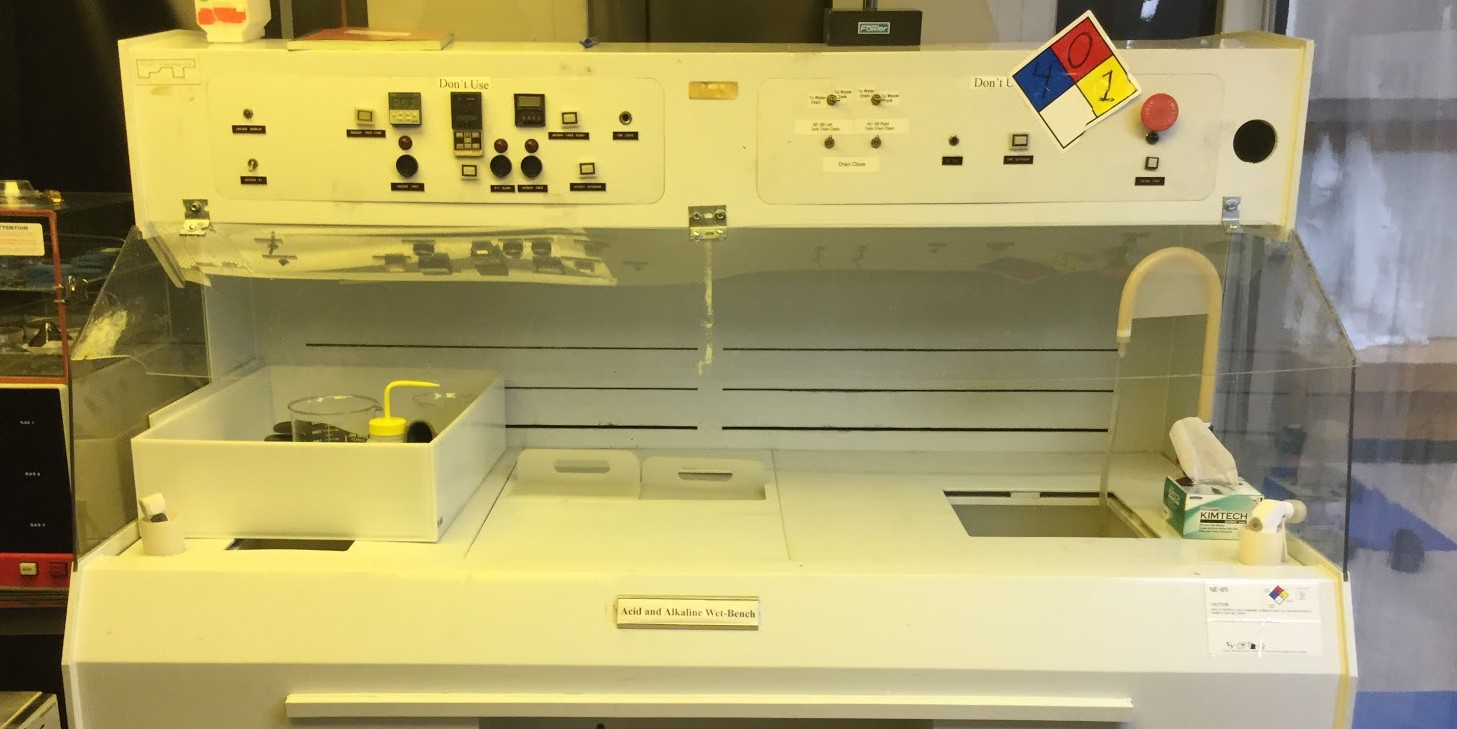
\includegraphics[width=0.5\textwidth]{plastic-hood.jpg}
\caption{Plastic hood for use with acids.}
\label{fig:plastichood}
\end{figure}



\section{Amorphous Ge Deposition}

Need information on the working principles of sputtering machine
\subsection{Principles of Sputtering}

\subsection{Operating Procedure}
The sputtering machine at USD is a Perkin-Elmer 4400 Sputtering System.

The operating procedure for the sputtering machine is complex and care is required to make sure the system maintains working order.
It is a complex system with multiple valves, controls, power supplies, vacuum systems, and pressure monitors that all work in conjunction to deposit a thin layer of amorphous germanium on the detector sample.
One key component of the system is a cryopump that uses pressurized helium gas to quickly vacuum the system to the proper pressure.
The cryopump system can be seen in Figure ~\ref{fig:sput-flow} as blue boxes with labels connected by green lines.
The green lines exchange the helium between the cold head connected to the vacuum chamber and the compressor located in the pump room.
Before the sputtering procedure can begin, the cryopump must be turned on to allow the cold head to cool from room temperature to approximately 20K.
The on/off switch for the compressor is located on the panel with the other valve toggles and is labeled as "HY-VAC PUMP"

Once the cryopump is cooled down to the proper temperature, the sputtering procedure can begin.
As seen in Figure ~\ref{fig:sput-flow}, there are multiple valves for opening and closing various gas and vacuum lines.
These valves are all pneumatically opened and closed so they require a constant supply of pressurized air at 60 psi.
This pressurized air is supplied by a large Kaeser SX 5 compressor located in the pump room and shown in Figure ~\ref{fig:comp-air}.
\begin{figure}[htpb]
\centering
\includegraphics[width=\textwidth]{comp-air}
\caption{Kaeser SX 5 compressor}
\label{fig:comp-air}
\end{figure}
The compressor is turned on or off by pressing the green or red button on the control interface shown on the top left side of the figure.
Once turned on, it will automatically increase in pressure until it reaches a set point around 100 psi.
The pressure out is then reduced or increased by adjusting the pressure regulator shown on the bottom left.
It is important to check the pressure often to make sure that it is sufficiently high for if it drops too low, valves will return to the default closed position.

Once the system has been supplied with pressurized air, the valves can be opened or closed and the system is ready to be operated.
The next step is to load the detector sample into the sputtering machine and prepare for deposition.
The sputtering system should always be kept under vacuum so before it can be opened it must be returned to standard atmospheric pressure.
This is done by opening the vent valve and filling the chamber with dry nitrogen.
The toggle switch for the vent valve is located at 'A' in Figure ~\ref{fig:sput-flow}.
The nitrogen in routed in from a tank located in a separate room behind the pump room and is kept at approximately 10 to 15 psi.

After the chamber has returned to atmospheric pressure it can be opened using a hydraulic lift system that is powered through the RF power generator.
The sample can now be carefully placed inside the chamber centering it under the amorphous germanium target as seen in Figure ~\ref{fig:sput-open}.
\begin{figure}[htpb]
\centering
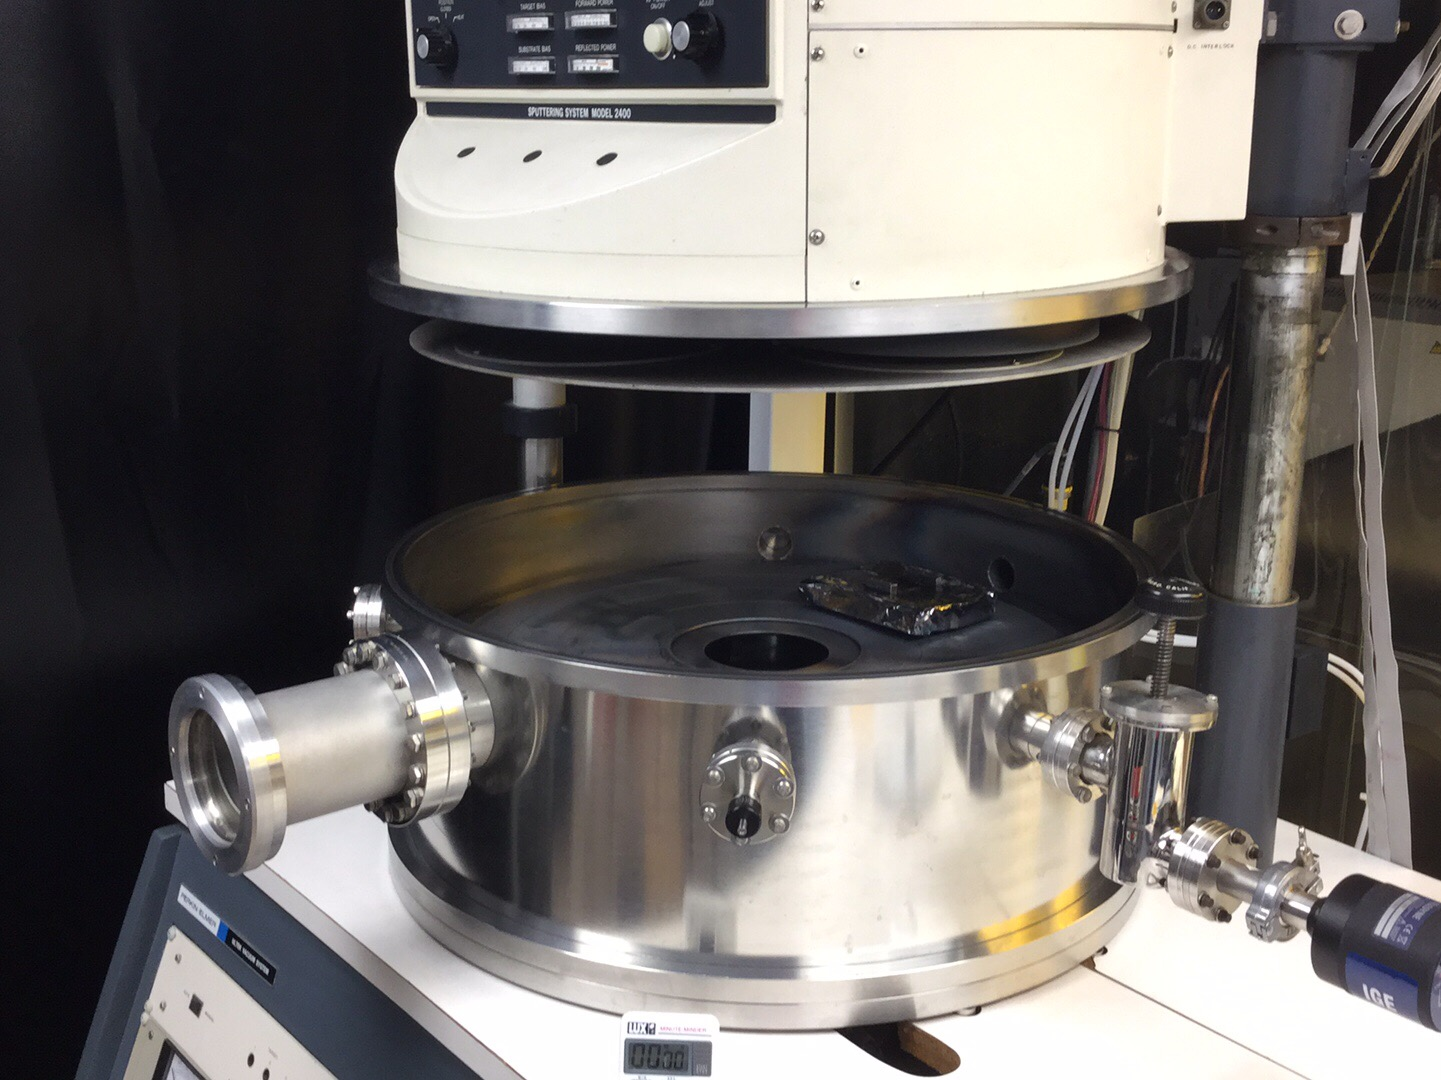
\includegraphics[width=0.6\textwidth]{sput-open.JPG}
\caption{Sputtering machine with chamber open}
\label{fig:sput-open}
\end{figure}
A jig is used to hold the detectors by the wings during the sputtering process.
It is designed to be adjustable, allowing for various detector sizes and geometries.
After the detector sample has been chemically etched it can be loaded onto the jig and then into the sputtering machine.

Once the sample is loaded the chamber can be closed and vacuum pumping can begin.
The first stage of pumping is done by a rough pump which takes the chamber from atmospheric pressure down to below 100 millitorr 
\begin{figure}[htpb]
\centering
\includegraphics[width=\textwidth]{water-cool}
\caption{Water chiller for cooling the sputtering machine and e-beam evaporator}
\label{fig:water-cool}
\end{figure}

\begin{sidewaysfigure}
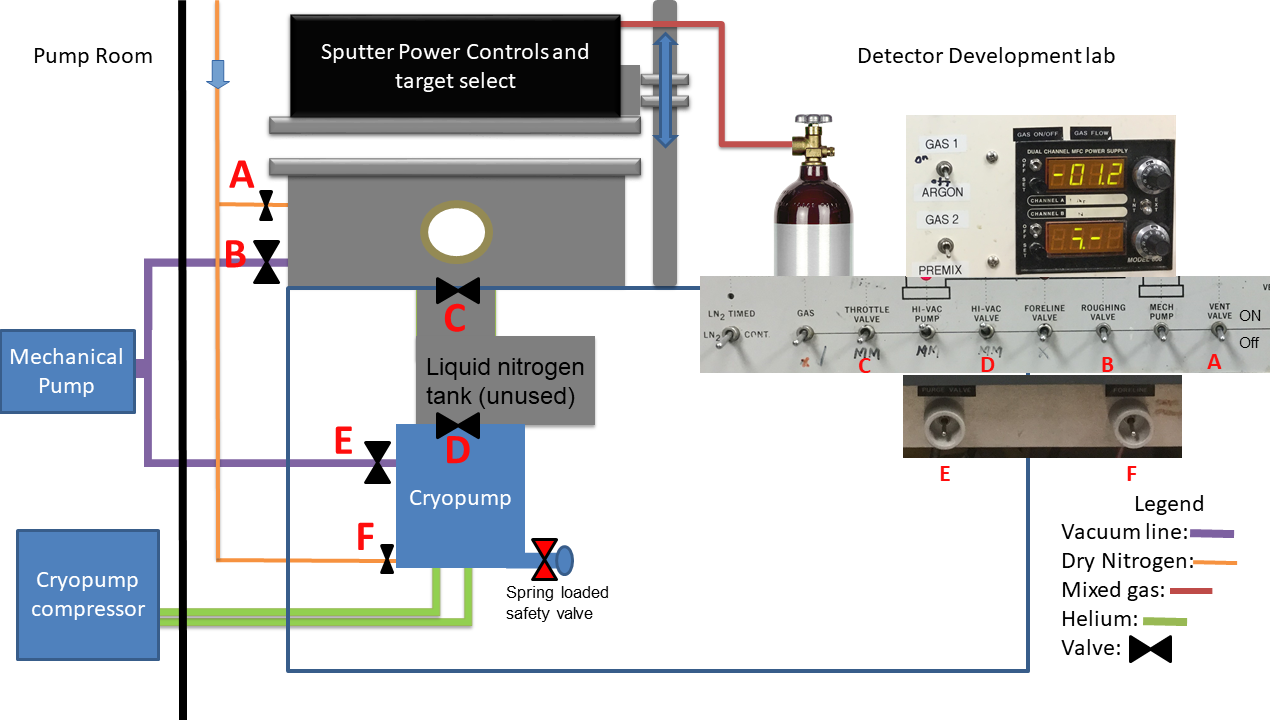
\includegraphics[width=\textwidth]{sput-flow}
\caption{This is a diagram of the Sputtering machine vacuum and gas system. Each valve is connected to a pressurized air line.}
\label{fig:sput-flow}
\end{sidewaysfigure}

\section{Aluminum Deposition}

\begin{sidewaysfigure}
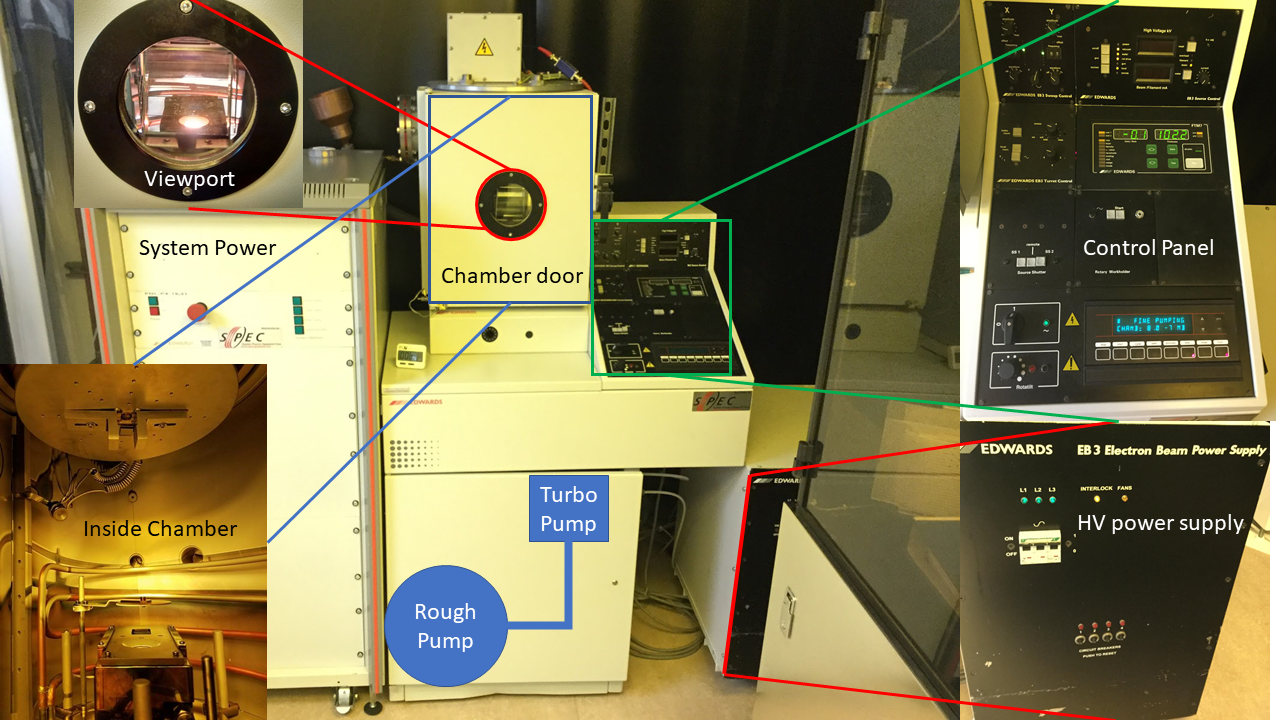
\includegraphics[width=\textwidth]{ebeam-flow}
\caption{This is a diagram of the of the electron beam machine.It is used to deposit aluminum onto the detector sample.}
\label{fig:ebeam-flow}
\end{sidewaysfigure}


\section{Final Steps}
